\section{Introduction}

In this chapter we develop a new model of frequency spectra, based upon the gradient of the frequency spectrum. We develop methods of band classification directly from compressive measurements, without reconstructing the signal as an intermediate step. This allows are system to operate at sampling rates below those predicted by Compressive Sensing theory - as the previous literature. We also show how by using this model, estimating frequency spectra is amenable to distributed reconstruction. We perform experiments on synthetic and real data (provided by OFCOM), which demonstrate our methods. We compare a distributed reconstruction and classification method with a centralised classification only method, and discuss their relative merits.

Compressive sensing makes the assumption that the signal being sensed is sparse. However we cannot always guarantee that the frequency spectrum will always be sparse: for example, should TVWS become widely utilised, the spectra will not be sparse. However, even for highly occupied spectra, the gradient of the spectrum will be sparse. This is because that TVWS spectra will feature bands with a flat power spectrum when occupied - or occupied bands will be well approximated by rectangular bands. Thus the PSD will feature abrupt changes in its gradient during transitions between occupied and unoccupied bands. This has previously been exploited by \cite{tian2006wavelet}. 

Reconstructing the spectrum from compressive measurements could take place at a fusion centre, but such communications are expensive. It is more efficient therefore to design distributed algorithms where CRs communicate with their neighbours to reach consensus on the reconstruction, given each nodes' private data. However, regularising the reconstruction process would require global co-ordination if Total Variation (TV) (the \(l_1\) norm of the gradient of the signal) regularisation was chosen. This is because the information about the gradient will be spread out amongst nodes in the network - these nodes may not necessarily be neighbours and so would not be able to share that information.

In this chapter we propose a different model for sensing the gradient of the frequency spectrum to \cite{tian2006wavelet} - a model which doesn't require Total Variation regularisation of the objective function. 

The structure of the chapter is as follows: in section \ref{sec:sig-model} we introduce the signal model and introduce a natural estimator of the signal using compressed measurements only. We demonstrate the results of this method on synthetic signals in \ref{sec:ci-results}, in section \ref{sec:dist-results} we show some results of the reconstruction quality of this model using the algorithm developed in chapter \ref{chap:dist-opt}. In section \ref{sec:ofcom-results}, we apply both of these methods to a larger dataset provided by OFCOM.
\clearpage

\section{Signal Model}\label{sec:sig-model}

Not all signals are sparse in an orthogonal basis: for example, many images are sparse in an over-complete dictionary (set of bases). In particular, TVWS frequency spectra, assumed to be sparse due to low occupancy - currently only digital TV is broadcast in these bands - may no longer be sparse once opportunistic radios begin operating in these frequencies. This is simply because as more bands are occupied, the sparsity assumption underlying modern recovery methods is violated. Thus any method that proposes to make decisions about spectral occupancy must contend with this. 

As an alternative we can aim to reconstruct the gradient of the spectrum, as we assume that transmissions are constant within a band. This is a viable alternative as, even if the frequency spectra is not sparsely occupied, transitions between constant power transmissions will be rare thus ensuring that the gradient of the frequency spectrum will be sufficiently sparse for modern sensing methods to be successful.

Consider the basis for \(\re^n\) defined by the function:

\begin{definition}[Heaviside Basis]
\begin{equation}
l_i\left(x\right) =
\begin{cases}
1 & \text{if } x \leq i \\
0 & \text{ otherwise } 
\end{cases}
\label{basis}
\end{equation}

That is, \(l_i\) is a left-hand step function. 

The basis (\ref{basis}) can be expressed as a matrix in \(\re^{n \times n}\), where basis vectors are written as rows of \(L_n\):

\begin{equation}
L_n = \begin{pmatrix}
 1 & 0 & 0 & 0  & 0 & \ldots & 0 \\
  1 & 1 & 0 & 0  & 0 & \ldots & 0\\
     1 & 1 & 1 & 0  & 0 & \ldots & 0  \\
    \ldots  \\
     1 & 1 & 1 & 1  & 1 & \ldots & 1 
\end{pmatrix}
\end{equation}
In general we write \(L_m\) for an \(m \times m\) matrix of this form.
\label{lower-L}
\end{definition}

\begin{lemma}
By direct computation, the inverse of \(L_n\) is:

\begin{equation}
D_n = \begin{pmatrix}
 1 & 0 & 0 & 0  & 0 & \ldots & 0 \\
  -1 & 1 & 0 & 0  & 0 & \ldots & 0\\
     0 & -1 & 1 & 0  & 0 & \ldots & 0  \\
    \ldots  \\
     0 & 0 & 0 & 0  & -1 & \ldots & 1
\end{pmatrix}
\end{equation}
In neural we write \(D_m = L_m^{-1}\) for an \(m \times m\) matrix of this form.
\label{inv-L}
\end{lemma}

\begin{definition}
We model our PSD signal \(g\) as a linear combination of the basis functions (\ref{basis}):

\begin{equation}
g\left(x\right) = \sum_i q_i l_i\left(x\right) = L^Tq
\label{basis-expansion}
\end{equation}

where \(q = (q_1, \ldots, q_n) \) are the coefficients in this basis expansion, and \(l_i\) are the rows of \(L\). Note that as defined, \(g\) is a column vector.
\end{definition}

\begin{proposition}
We can recover the coefficients \(q\) from \(g\) easily since:
\begin{equation}
D_n^Tg = q
\end{equation}
\label{def:a}
\end{proposition}
\begin{proof}

\begin{align}
D_n^Tg &= D_n^T L_n^T q \\
&= \left(L_nD_n\right)^Tq \\
&= q
\end{align}

as \(L_nD_n = I_n\).

\end{proof}


\begin{definition}
We can define a matrix representation for the set of basis vectors \(l_i\), by taking all inner products between all pairs of basis vectors:

\begin{equation}
F_{n, ij} = \langle l_i, l_j \rangle
\end{equation}

This matrix has the representation:

\begin{equation}
F_{n, ij} = \min(i,j)
\end{equation}

An example of such a matrix is:

\begin{equation}
F_n= \begin{pmatrix}
 1 & 1 & 1 & 1  & 1 \\
  1 & 2 & 2 & 2  & 2\\
     1 & 2 & 3 & 3  & 3  \\
    1 & 2 & 3 & 4  & 4  \\
     1 & 2 & 3 & 4  & 5 
\end{pmatrix}
\label{def:Fmtx}
\end{equation}
\end{definition}

\begin{theorem}
This matrix is invertible since:

\begin{equation}
\det(F_n) = 1
\end{equation}
\end{theorem}
\begin{proof}
Consider the matrix \(F_n\). Subtract the (\(n-1\))th column from the \(n\)th. This will not change the value of the determinant of \(F_n\) We obtain a matrix with \(0\) on the final column except the entry \(F_n(n,n) = 1\). 


\begin{equation}
F_n= \begin{pmatrix}
 1 & 1 & 1 & 1  & 0 \\
  1 & 2 & 2 & 2  & 0\\
     1 & 2 & 3 & 3  & 0  \\
    1 & 2 & 3 & 4  & 0 \\
     1 & 2 & 3 & 4  & 1 
\end{pmatrix}
\end{equation}

Since the top \((n-1) \times (n-1)\) is \(F_{n-1}\) we find that 

\begin{equation}
\det(F_n) = 1 \times \det(F_{n-1})
\end{equation} 

By recursion and \(\det(F_1) = 1\) we have \(\det(F_n) = 1\).

\end{proof}

This matrix can be factorised as \(F_n = L_nL_n^T\).

From this it follows that

\begin{equation}
F_n^{-1} = \begin{pmatrix}
 2 & -1 & 0 & 0  & 0 &\ldots & 0 \\
  -1 & 2 & -1 & 0  & 0  &\ldots & 0\\
     0 & -1 & 2 & -1  & 0  &\ldots & 0  \\
    \ldots  \\
     0 & 0 & 0 & 0 &-1 & \ldots & 1 
\end{pmatrix} = D_n^TD_n
\end{equation}

To find the \(q_i\), we correlate (take the inner product of) the signal against the basis \eqref{basis}.

\begin{definition}[Inner Product]
We define the inner product between two vectors as follows:

\begin{equation}
\langle u, v \rangle = u^T v = \sum_i u_i v_i
\end{equation}	
where \(u_i, v_i\) are the components of the vectors \(u,v\) in the \(i^{th}\) direction with respect to some orthonormal basis vectors \(e_i\).

In general, we have to adapt this for basis vectors which are not orthogonal, for example:

\begin{equation}
\tilde{u} = \sum_i a_i l_i\left(x\right) = L_n^T a
\end{equation}

\begin{equation}
\tilde{v} = \sum_i b_i l_i\left(x\right) = L_n^T b
\end{equation}

Then, the inner product can be expressed as:

\begin{equation}
\langle \tilde{u}, \tilde{v} \rangle = a^T L_n L_n^T b = a^T F_n b
\end{equation}	

\end{definition}

\begin{definition}[Cumulative Sum]
We can express the inner product between the signal \(g\) and the set of basis vectors as:

\begin{equation}
h_j = \langle g, l_j \rangle
\label{eq:h-est}
\end{equation}

this is a useful quantity, as it is the cumulative sum of the signal \(g\):

\begin{align}
h_j &= \langle g, l_j \rangle \\
&= \sum_x g\left(x\right) l_j\left(x\right) \\
&= \sum_x \sum_i q_i l_i\left(x\right) l_j\left(x\right) \\
&= \sum_i q_i \sum_x l_i\left(x\right) l_j\left(x\right) \\
&= q_i \langle l_i, l_j\rangle \\
\end{align}

In matrix language \(h = F q^T\). This is the inner product between the signal \(g\) and the basis functions \(l_i\).
\end{definition}

\begin{example}[Single Rectangle]
\label{ex:single-rect}
Consider a signal \(g\left(x\right) \in \re^n\) which is 

\begin{equation}
g\left(x\right) =
\begin{cases}
1 & \text{if } \frac{n}{4} \leq x < \frac{3n}{4} \\
0 & \text{ otherwise } 
\end{cases}
\end{equation}

in the basis defined by \eqref{basis}, this function can be expressed as:

\begin{equation}
g\left(x\right) = L_n^Tq
\end{equation}

with 
\begin{equation}
q_i =
\begin{cases}
-1 & \text{if } i = \frac{n}{4} \\
1 & \text{if } i = \frac{3n}{4} \\
0 & \text{ otherwise } \\
\end{cases}
\end{equation}

\end{example}

\begin{algorithmic}[1]
 %\SetAlgoLined % For previous releases [?]
 \Procedure{Estimate Occupancy}{$y$, $A$, $k$}
 \State{\textbf{Inputs}: A set compressive measurements \(y\), a measurement matrix \(A\), and an integer \(k\)}
 \State{\textbf{Returns}: \(\hat{g}\), an estimate of the occupancy of a frequency spectrum.}
 \\
Calculate \(g=A^ty\)
 \\
Choose a set of indices using procedure Index Pursuit
\\
 Between the indices of \(g\) take the average.
 \\
   	For each piece between the \(k\) changepoints, do a t-test to determine whether the signal is noise, or a transmission.
   	\EndProcedure
\end{algorithmic}


\begin{algorithmic}[1]
 %\SetAlgoLined % For previous releases [?]
 \Procedure{Index Pursuit}{}
 \State{\textbf{Inputs}: \(g=A^t y\), \(L\), \(F^{-1}\), \(k\)}
 \State{\textbf{Returns}: A set \({j}_{i=1}^k\) of indices}
 \\
 Set \(z = A^ty\), \(\mathrm{inds} = \varnothing \)
 \\ For \(i=1:k\):
 \\ Calculate \(u = Lz\), and \(\alpha = F^{-1}u\)
 \\ Find \(\max_i|\alpha|\)
 \\ Set \(z = z - \alpha_i e_i\)
 \\ Set \(\mathrm{inds} = \mathrm{inds}+i\)
 \EndProcedure
\end{algorithmic}


\begin{figure}[h]
\centering
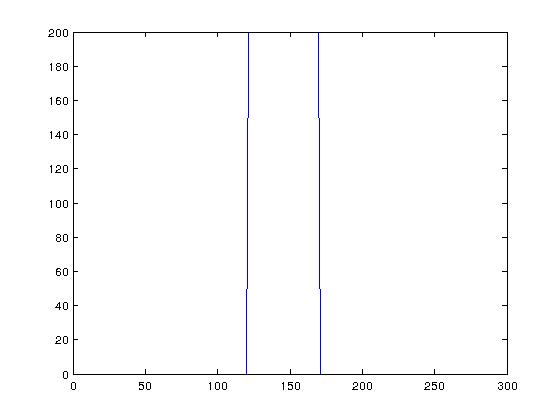
\includegraphics[height = 7.3 cm]{g.jpg}
\caption{A single rectangle signal, simmilar to example \ref{ex:single-rect}. This signal is used as an illustrative demonstration for the method developed in this chapter.}
\label{fig:rectangle}
\end{figure}

We now describe the procedure \ref{alg:single-slot}, in detail. Given a set of compressive measurements: 

\begin{equation}
y = Ag = AL_n q^T
\end{equation}
\\
where \(A \in \re^{m \times n} \), \(A_{ij} \sim \mathcal{N}\left(0,1/m\right)\), we then compute 
\begin{equation}
\langle y, Al_i\rangle = q_j  l_j^TA^tAl_j \sim \frac{q_j}{m} \langle l_j, l_i \rangle
\label{key-step}
\end{equation}
for the set of basis vectors \(l_1 \ldots l_n\) i.e. the estimator from the previous section, corresponding to this set of basis functions \eqref{eq: compressive-estimator}. 

\begin{remark}
This is the key step in this procedure. The relation 

\begin{equation}
\langle y, Al_i\rangle = q_j  l_j^TA^tAl_j \sim \frac{q_j}{m} \langle l_j, l_i \rangle
\end{equation}

is valid because of the RIP \eqref{def:RIP} from chapter \ref{chap:cs}. We are using the fact that the matrix \(A^TA\) is \(\delta\)-close to an isometry (where \(\delta\) is the RIP constant of \(A\), along with the result of theorem \eqref{thm:wishart-mean}, to estimate the vector \(h\).

\end{remark}
We then form the vector 

\begin{equation}
\hat{h} = m \sum_i \langle y, Al_i\rangle l_j \sim h
\label{ss-estimator}
\end{equation}

Again, this relation (\(\sim\)) is based on the same reasoning as the previous equation \eqref{key-step}.

An example can be seen in figure \ref{fig:hhat}, for a matrix \(A \in \re^{200 \times 300}\).

\begin{figure}[h]
\centering
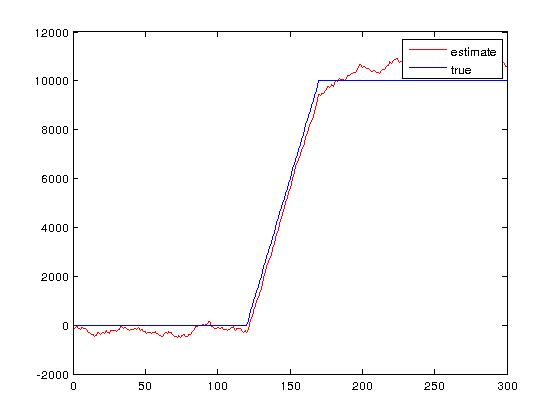
\includegraphics[height = 7.3 cm]{hhat.jpg}
\label{fig:hhat}
\caption{An example of the estimate \(\hat{h}\) for a single rectangle signal (in red) compared to the true cumulative vector \(h\) (in blue). Note how the estimate tracks the true signal, with little deviation.}
\end{figure}

\clearpage

\section{Results for Compressive Inference}
\label{ci-results}

In this sections we report experiments applying the compressive inference methods described in section \ref{sec:sig-model} to a synthetic dataset. We created in signal in \(\re^{1000})\) (pictured in figure \ref{ci-sig}), and ran the sensing and classification process at a variety of SNRs and undersampling points. Results are averaged over 100 runs, in each SNR regimen and at each undersampling point.

These results are collected in figures \ref{different_k}, \ref{different_k_4.5}, \ref{different_k_10.5}, and \ref{different_k_18}. Collectively these figure show that the performance of algorithm \ref{alg:single-slot} degrades with both undersampling and a worsening radio environment. We remark that the algorithm withstands substantial noise before degrading significantly, at all levels of undersampling. For example with an SNR of -10dB, a classifier with 1\% of the samples is still 90\% accurate. In the more favourable SNR regime of -4.5dB, a classifier with 1\% of the samples is still 95\% accurate.

Figures \eqref{snrauc} and \eqref{snrauc_pan} encapsulate and corroberates this insight. In particular in figure \eqref{snrauc} at all levels of undersampling the performance of algorithm \ref{alg:single-slot} degrades with worsening radio environments - this is evidenced by lower AUC for each curve as the SNR decreases. However, this is 


\begin{figure}[h]
\centering
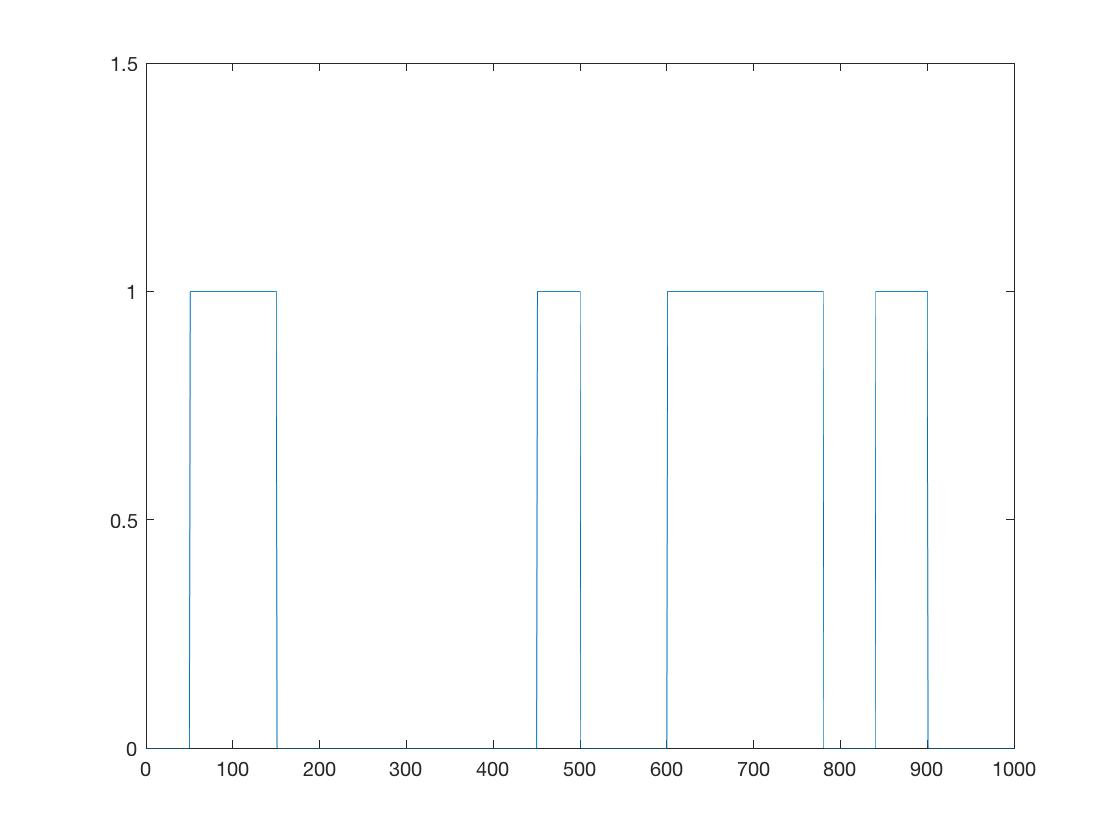
\includegraphics[height = 7.3 cm]{ci-sig.jpg}
\caption{Synthetic signal used for experiments in this section}
\label{ci-sig}
\end{figure}


\begin{figure}[h]
\centering
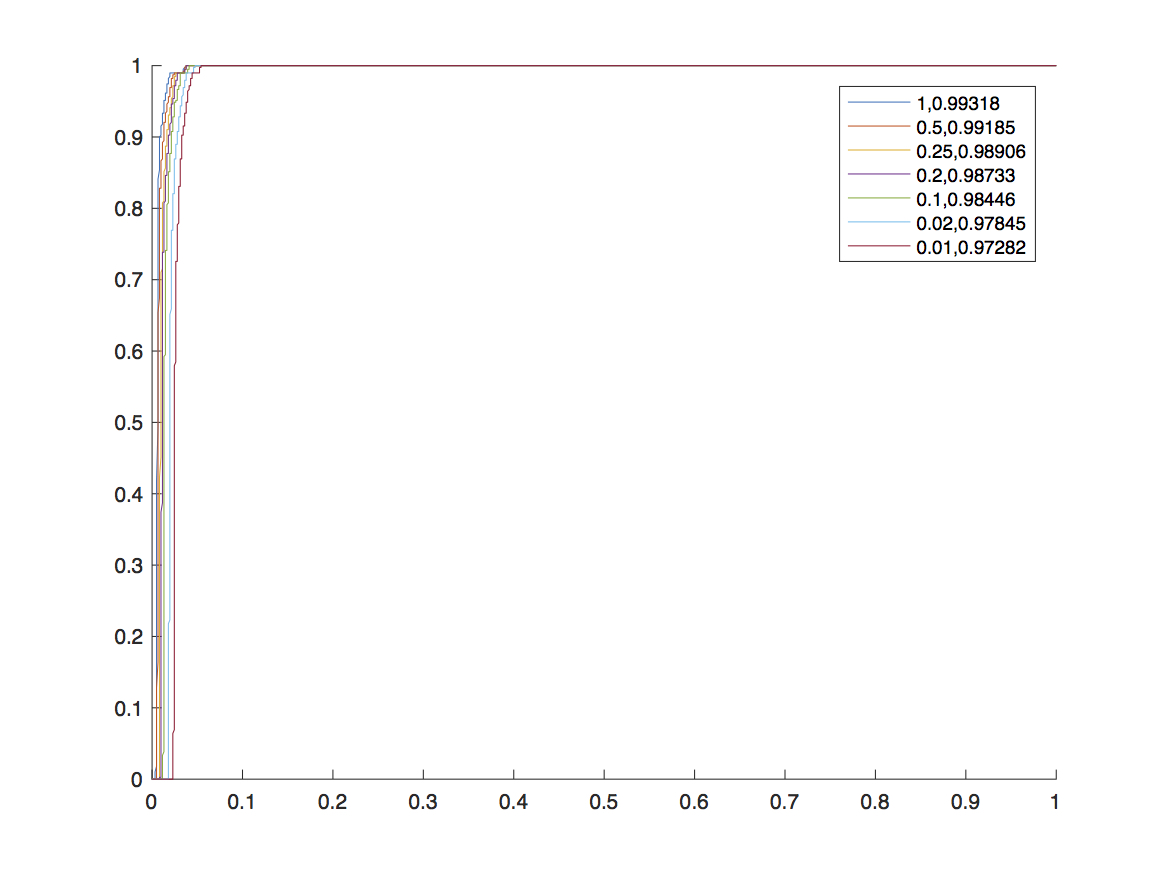
\includegraphics[height = 7.3 cm]{one-shot-different-k.jpg}
\caption{ROC curves for the single-shot algorithm (as outlined in table \ref{alg:single-slot}), for a  reconstruction of a  the signal in \ref{ci-sig}. The first number in the legend is the ratio \(m/n\), whilst the second is the area under the curve.}
\label{different_k}
\end{figure}


\begin{figure}[h]
\centering
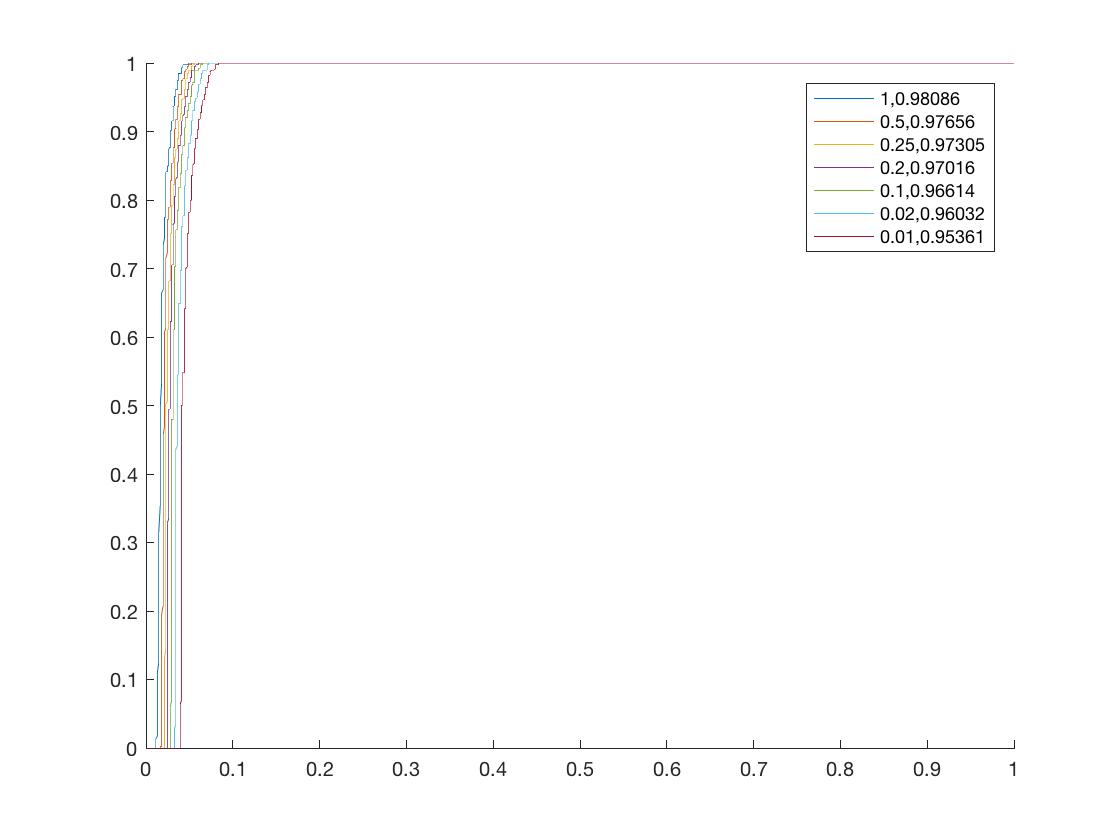
\includegraphics[height = 7.3 cm]{single_shot_snr_-45.jpg}
\caption{ROC curves for the single-shot algorithm (as outlined in \ref{alg:single-slot}), for a signal in \(\re^{1000}\), with noise added at an SNR of \(-4.5\)dB. The first number in the legend is the ratio \(m/n\), whilst the second is the area under the curve.}
\label{different_k_4.5}
\end{figure}

\begin{figure}[h]
\centering
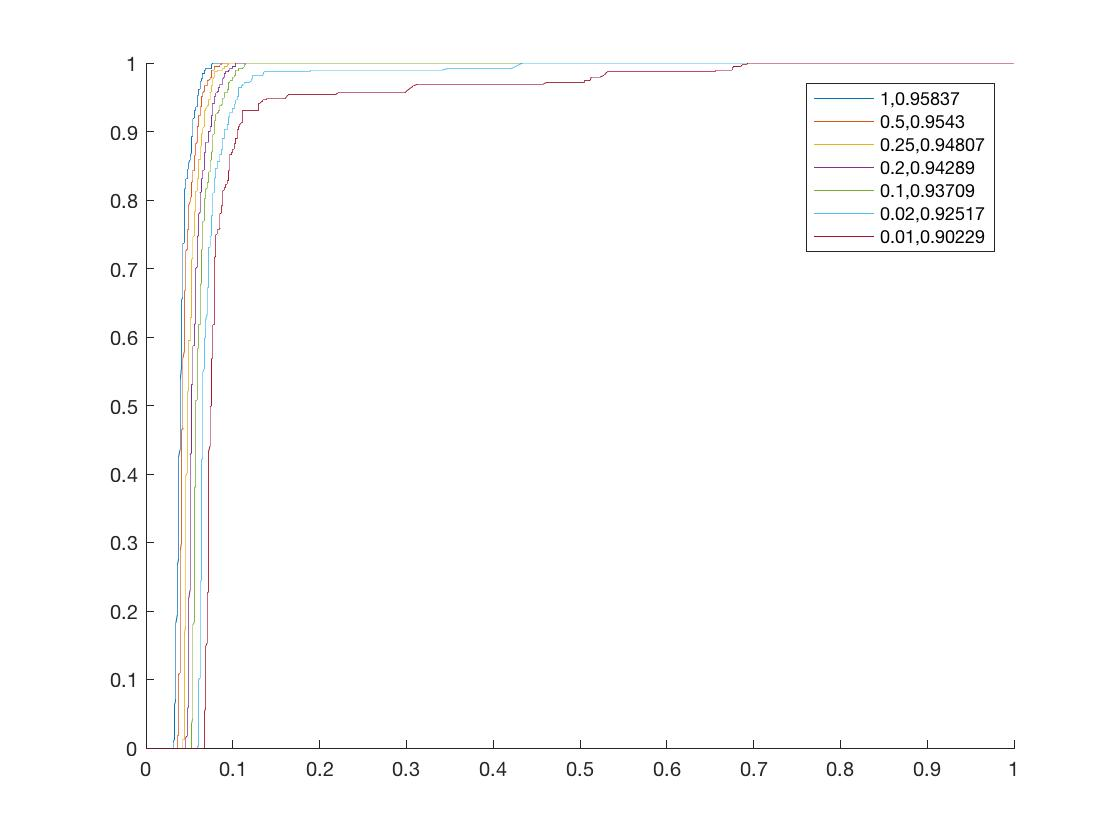
\includegraphics[height = 7.3 cm]{single_shot_snr_-105.jpg}
\caption{ROC curves for the single-shot algorithm (as outlined in \ref{alg:single-slot}), for a signal in \(\re^{1000}\), with noise added at an SNR of \(-10.5\)dB. The first number in the legend is the ratio \(m/n\), whilst the second is the area under the curve.}
\label{different_k_10.5}
\end{figure}

\begin{figure}[h]
\centering
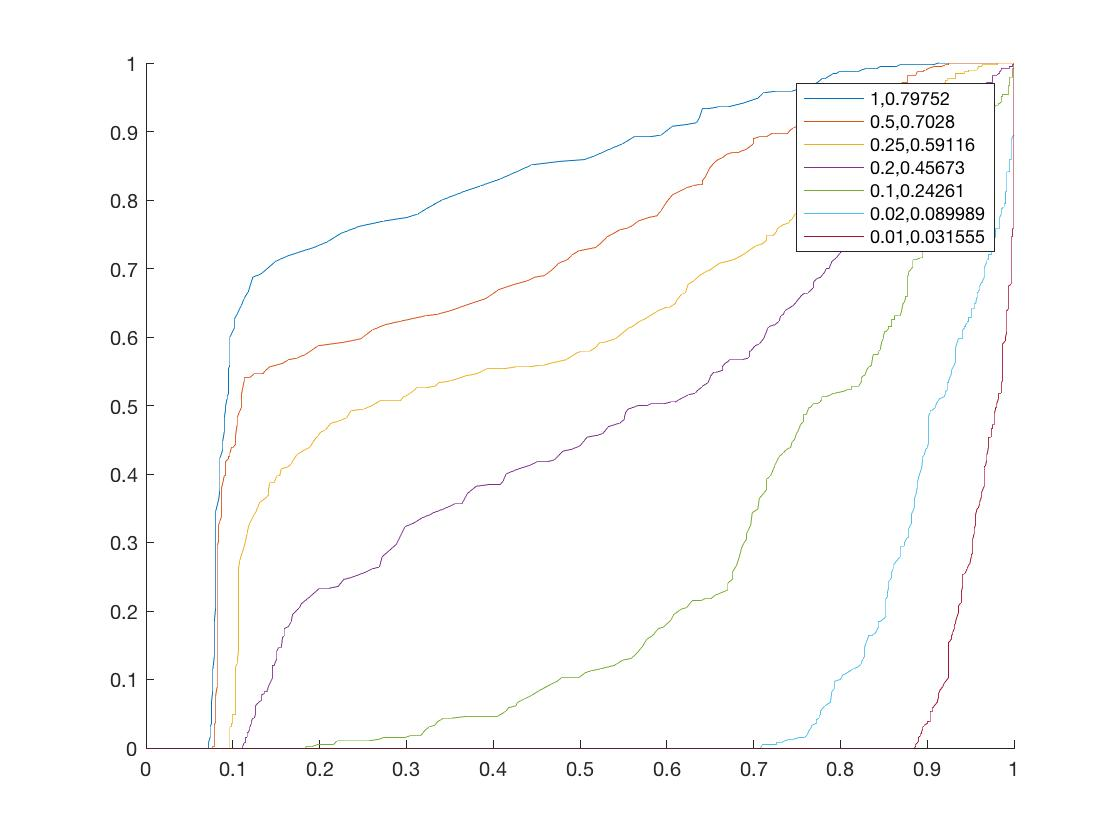
\includegraphics[height = 7.3 cm]{single_shot_snr_-18.jpg}
\caption{ROC curves for the single-shot algorithm (as outlined in \ref{alg:single-slot}), for a signal in \(\re^{1000}\), with noise added at an SNR of \(-18\)dB. The first number in the legend is the ratio \(m/n\), whilst the second is the area under the curve.}
\label{different_k_18}
\end{figure}

\begin{figure}[h]
\centering
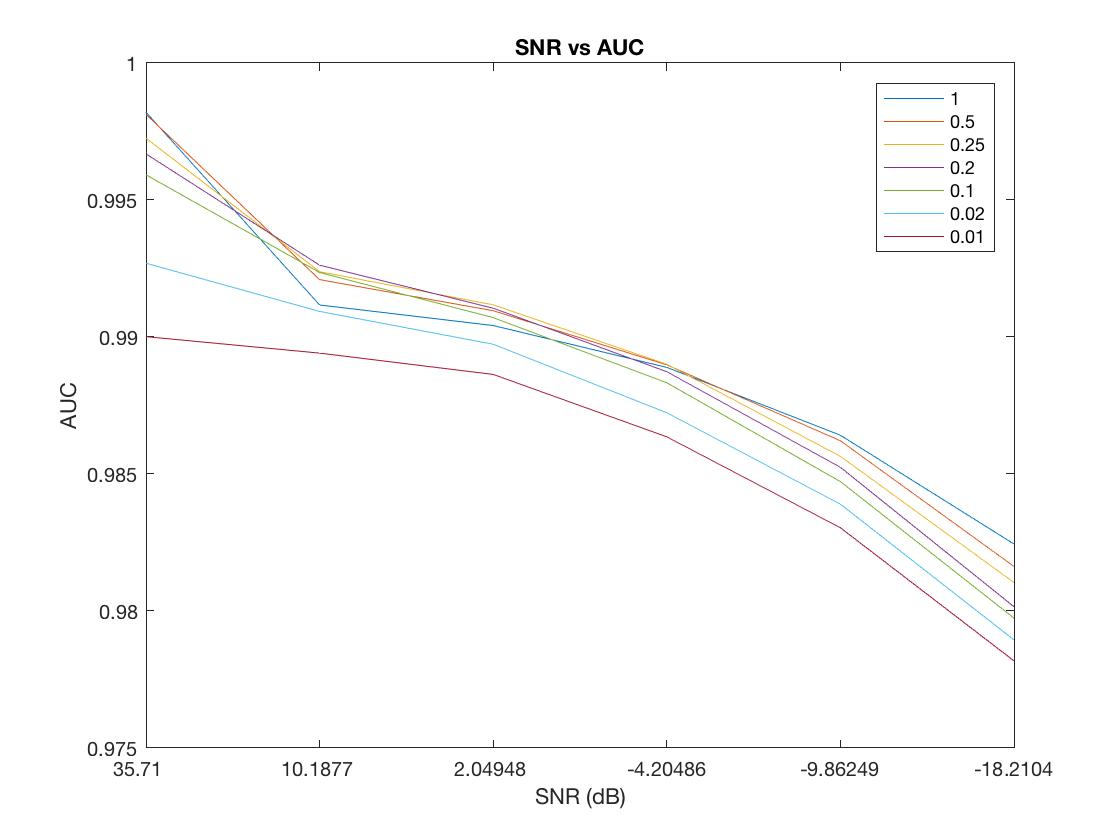
\includegraphics[height = 7.3 cm]{snrvsauc.jpg}
\caption{SNR vs AUC for different levels of undersampling (as indicated in the legend)}
\label{snrauc}
\end{figure}

\begin{figure}[h]
\centering
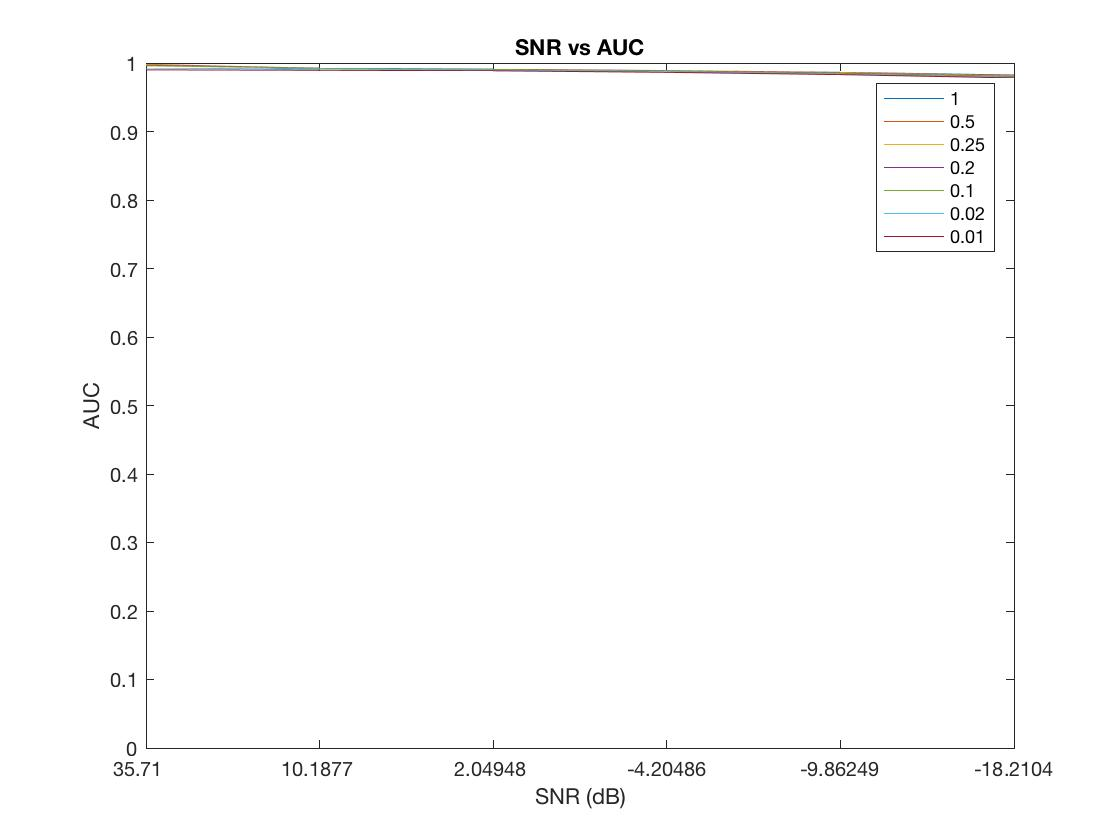
\includegraphics[height = 7.3 cm]{snrvsauc_zoomedout.jpg}
\caption{SNR vs AUC for different levels of undersampling (as indicated in the legend), this time zoomed out from figure \eqref{snrauc}}
\label{snrauc_pan}
\end{figure}

\clearpage

\subsection{Benchmarking the Algorithm}
In this section we benchmark the algorithm (\ref{alg:single-slot}), against a version of the algorithm provided with the accurate change points (as inferred in \ref{alg:single-slot} by \ref{alg:index_pursuit}). To our knowledge there is no similar prior art, applying similar methods to TVWS data. This is why we have decided to benchmark the algorithm against a hypothetical version which has access to the correct changepoints. Figures \ref{oracle-compare} and \ref{oracle-compare} show ROC curves for various undersampling levels using  the synthetic signal \ref{ci-sig}, for algorithm \ref{alg:single-slot} and \ref{alg:single-slot} with oracle changepoints. Each curve was produced after 100 runs. The curves clearly show that the performance of the algorithm matches that of the oracle.

\begin{figure}[h]
\centering
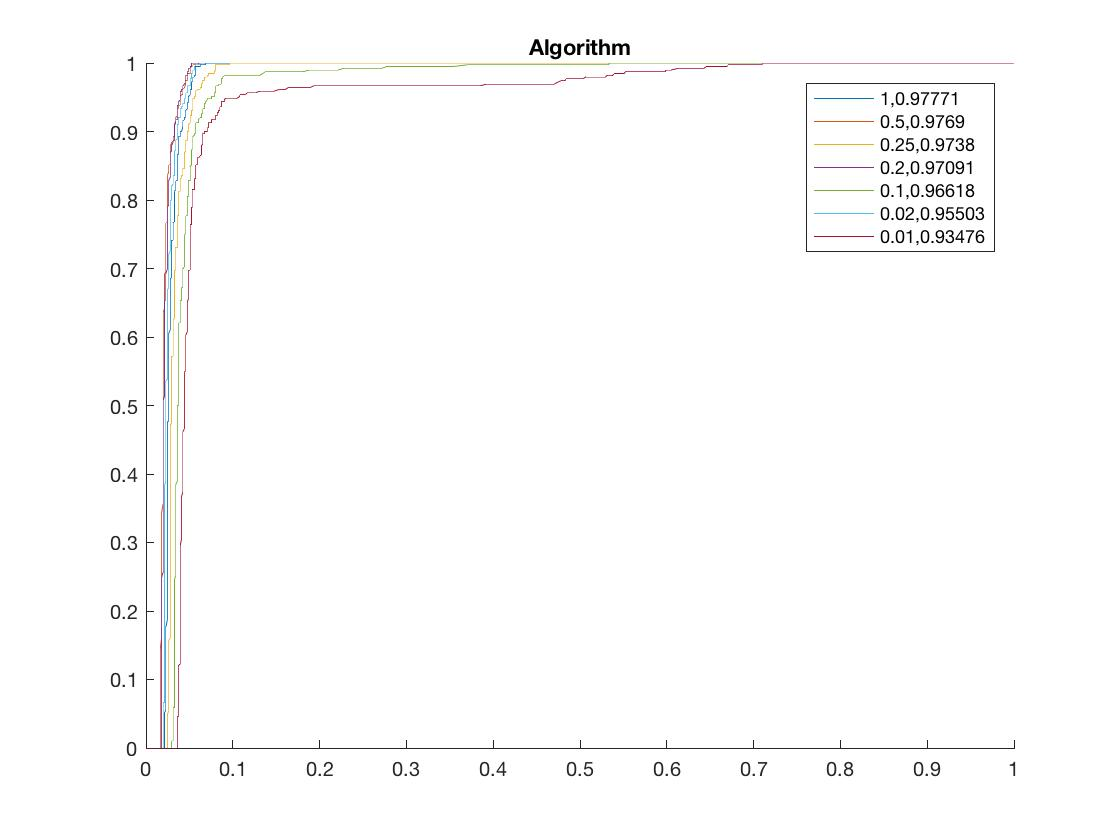
\includegraphics[height = 7.3 cm]{smashed_filt_10.jpg}
\caption{ROC curves for the single-shot algorithm (as outlined in table ,l;/l\ref{alg:single-slot}), for a signal in \(\re^{1000}\), with noise added at an SNR of \(-10\)dB. The first number in the legend is the ratio \(n/m\), whilst the second is the area under the curve.}
\label{oracle-compare}
\end{figure}

\begin{figure}[h]
\centering
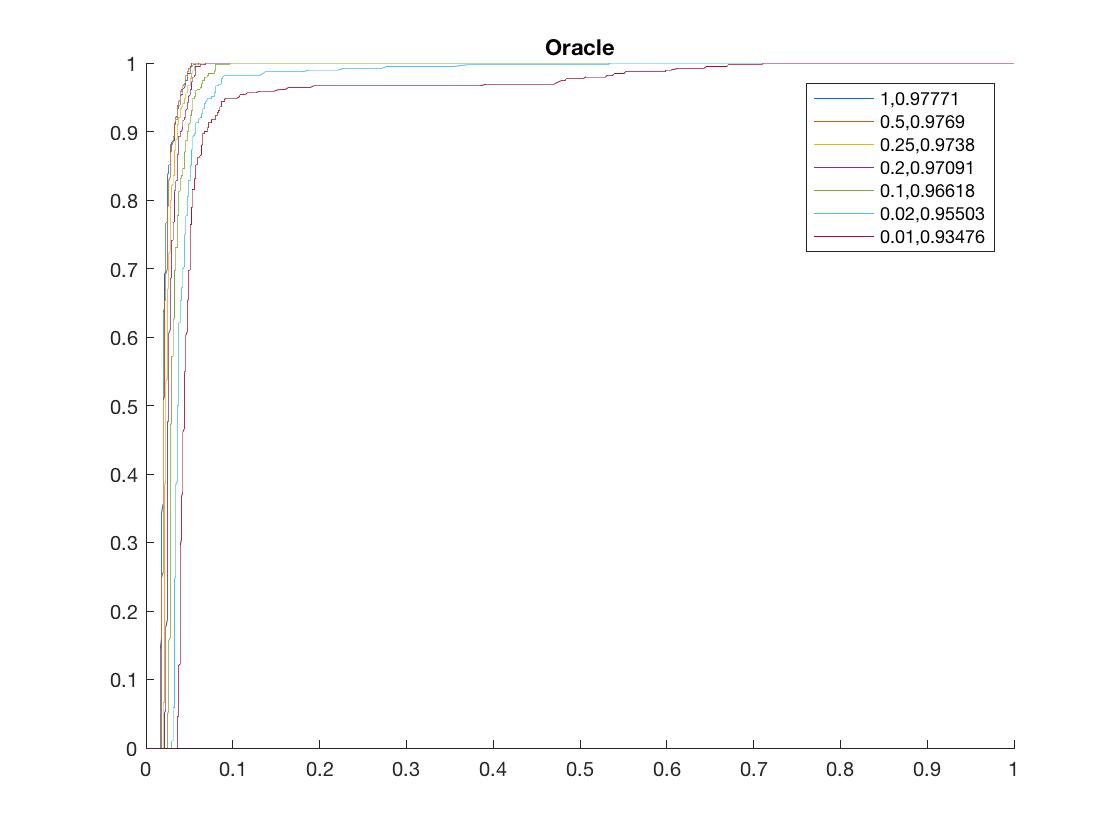
\includegraphics[height = 7.3 cm]{oracle_10.jpg}
\caption{ROC curves for the single-shot algorithm with correct changepoints, for a signal in \(\re^{1000}\), with noise added at an SNR of \(-10\)dB. The first number in the legend is the ratio \(n/m\), whilst the second is the area under the curve.}
\label{oracle}
\end{figure}

\clearpage

\section{Results for Distributed Sensing}
\label{sec:dist-results}
The model described in section \eqref{sec:sig-model}, equation \eqref{system} was simulated. The signal \(g \in \re^{300} \) was composed of 3 rectangular pulses, mimicking primary user signals in TVWS, as shown in figure \eqref{different_sigs} (a). The signal was put through a Rayleigh channel, before being sensed by the nodes. The network was generated as a random geometric graph in \([0,1] \times [0,1]\), with 50 nodes. If the network wasn't connected, it was redrawn. 200 mixing patters were drawn i.i.d from a \(\mathcal{N}\left(0, \sigma^2 I_{300} \right) \) distribution, with \(\sigma^2 = 1/200\), to from the matrix \(A\in  \re^{200 \times 300}\).

Monte Carlo simulations were performed at 18 \(\sigma^2_n\) values ranging from 1 to 10 and the expected Mean Squared Error (MSE) of solutions of a centralised ADMM solver and a our distributed solver \ref{sec:algo-lasso} were calculated over 500 repetitions with 1200 iterations (\(k\)) per repetition.

The MSE was calculated as follows:

\begin{equation}
\frac{\vectornorm{L^tz^k - g^*}}{\vectornorm{g^*}}
\end{equation}

where \(z^k\) is the result of the algorithm at iteration \(k\), and \(g^*\) is the optimal solution.

The SNR for each repetition was calculated as

\begin{equation}
\frac{\vectornorm{g^*}}{\vectornorm{w}}
\end{equation}

and averaged over the 500 repetitions. The results are shown in figure \eqref{msevssnr0}. Following \cite{Chen1998}, for each repetition we chose 

\begin{equation}
\lambda = \sqrt{2\sigma^2_n\log{n}}
\end{equation}

The error bars indicate the empirical variance across the 500 repetitions.

These results indicate that for both the centralised and distributed solvers, their performance degrades as the noise power increases in a roughly log-linear fashion. The performance of the distributed algorithm is consistently worse than the centralised version, this contrasts with results from \cite{bazerque2008}; this is due to the differing sparsity models: \cite{bazerque2008} use a joint space and frequency model for the sparsity, and as such observe an spatial averaging out of noise when using a distributed solver. The performance of DADMM is within the error bars of the centralised version at low SNR, and gap in performance between the two versions is no more than \(10^{-2}\). Even at relatively lower SNRs both solvers reach a solution within \(10^{-1}\) of the optimal (as measured by normalised MSE), which will be adequate for the task of spectrum sensing. For example the reconstructions in figures \eqref{different_sigs} (c) and (d) show realisations of the reconstruction from DADMM with \(\sigma^2_n = 5\) and \(\sigma^2_n = 20\) respectively. It is still possible to distinguish the occupied bands from unoccupied frequencies for both reconstructions.

The distributed algorithm has consistently larger variance, than the centralised solver at all SNRs. This is due to individual nodes only having access to a subset of the data to perform calculations on: the variance will be proportional to the square-root of number of data samples at each node, which are fewer than the total number of samples available to the centralised solver. 

In figure \eqref{fig:differentLambda}, we plot the progress of DADMM along the solution path for a variety of regularisation parameters \(\lambda\). The y-axis is the relative (unormalised) MSE between the optimal solution and the current iteration, and the x-axis is the iteration number. We note that for a fixed \(\lambda\) there is a single unique optimal solution, which DADMM converges to (in the sense of stationary error between consecutive iterations). This solution may not be attained in the allotted number of iterations, as the rate of convergence is determined by \(\lambda\), \(\rho\) and the eigenvalues of the Laplacian of \(G\). The paper \cite{shi2014linear}, proves linear convergence for DADMM, with explicit expressions for the rate. In particular the rate convergence of DADMM is affected by the choice of \(\lambda\): smaller \(\lambda\) corresponds to slower convergence - this is intuitive as solutions with fewer non-zero components should require fewer iterations to fully specify. Notice that for some \(\lambda\)s the solution path exhibits phenomenological  behaviour similar to damped oscillations: this phenomena has been explored in \cite{nishihara2015general} and \cite{su2014differential}.  

\begin{figure}[h]
\centering
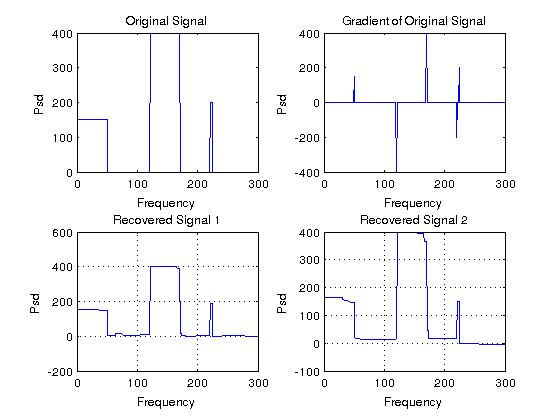
\includegraphics[height = 7.3 cm]{signal_and_recovery.jpg}
\caption{Left to right: (a) The original signal. (b) The gradient \eqref{def:a} of the original signal. (c) Recovery using DADMM, 1000 iterations, \(\sigma^2_n = 5\). (d) Recovery using DADMM, 1000 iterations, \(\sigma^2_n = 20\)  }
\label{different_sigs}
\end{figure}

\begin{figure}[h]
\centering
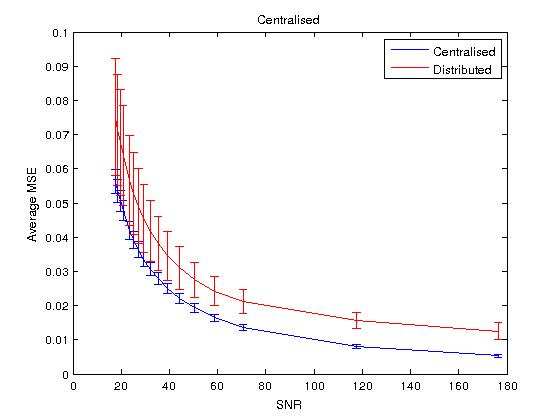
\includegraphics[height = 7.3 cm]{Cent_Vs_Distrib_snr.jpg}
\caption{MSE vs SNR for the sensing model showing the performance of distributed and centralised solvers. The performance of DADMM is consistently within \(10^{-2}\) of ADMM, and within the error bars of ADMM at low SNRs. The variance of estimates produced by DADMM is larger than ADMM, due to nodes performing computations on a subset of data. Both estimates are consistently within \(10^{-1}\) of the optimal solution, which is sufficient to classify occupied bands.} 
\label{msevssnr0}
\end{figure}

\begin{figure}[h]
\centering
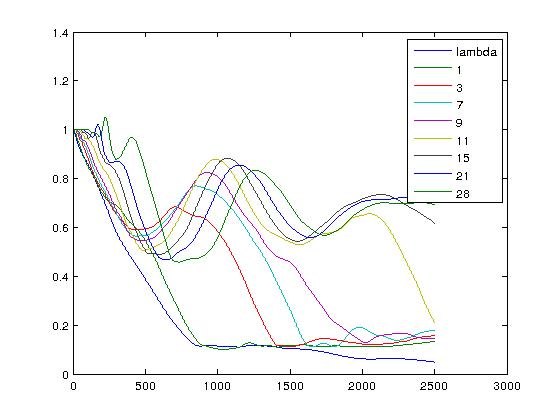
\includegraphics[height = 7.3 cm]{continuations_errors.jpg}
\caption{The progress of the distributed solver as a function of the number of iterations, with different values of the regression parameter \( \lambda \). For a fixed \( \lambda \) there is a single unique optimal solution, with higher \( \lambda \) favouring sparser solutions. The convergence of DADMM is slowed by smaller \( \lambda \). This is intuitive: solutions with fewer non-zero components should be identified in fewer iterations.}
\label{fig:differentLambda}
\end{figure}

\clearpage

\section{Results on OFCOM data}
\label{ofcom-results}

This section applies the methods of chapters \ref{chap:dist-opt} and \ref{chap:rect-basis}, specifically algorithms \ref{dadmm_algo_lasso}, and \ref{alg:single-slot} to a data set of TVWS measurements captured by OFCOM in the band 440-780MHz. The OFCOM dataset was taken in Southwark, UK during May 2014.

This section is organised as follows: we first describe the dataset in detail, and show example PSD captures for it, then we show results of the distributed estimation algorithm (presented in chapter \eqref{chap:dist-opt}), with estimation in the Heavyside basis. This algorithm is performed over a network of nodes, and reconstructs the sensed PSD via an iterative denoising procedure derived from the LASSO functional. It should be noted that this is the largest experiment of its kind: previous work has featured experimental results on far smaller datasets, or featured algorithms who's steps took considerably longer to reach an acceptable solution. We compare results produced by our algorithm to results from cooperative algorithms, and discuss the relative performance in terms of reconstruction quality, classification accuracy and algorithm speed. 

We then present results of the techniques outlined earlier in in this chapter \eqref{chap:rect-basis}, specifically algorithms \ref{alg:single-slot} on the OFCOM data set. This algorithm aims at classifying the signal directly from compressive measurements without reconstructing the signal as an intermediate step. The major feature of this methods is that classification can still be done accurately with severe undersampling.

\subsection{Data Set}

This data set was kindly supplied by OFCOM, and is of the 440-790 MHz TVWS band, with a resolution of 25 kHz. This is 1,048,575 data points, or 80 captures of the TVWS band. A single snapshot of the TVWS band is 10,000 data points,  The data set is 15.7 MB in size and was captured at Riverside House, Southwark, London, over a period of 1 hour in June 2014. 

There was no ground truth signal provided with the data set, so there is no way to quantitatively asses the goodness of our methods on this dataset. However, since the algorithms have been shown to perform well on suitable synthetic data, we be live that the results obtained in this section are valid.

\subsection{Results: Distributed Estimation with Heaviside Basis}

This subsection shows some examples of recovery of the OFCOM data with the DADMM-Lasso algorithm, as described in chapter \ref{chap:dist-opt}. Each example is with a different value of \(\lambda\) the regularisation parameter, which trades off recovery accuracy with recovery sparsity.

\begin{figure}[h]
\centering
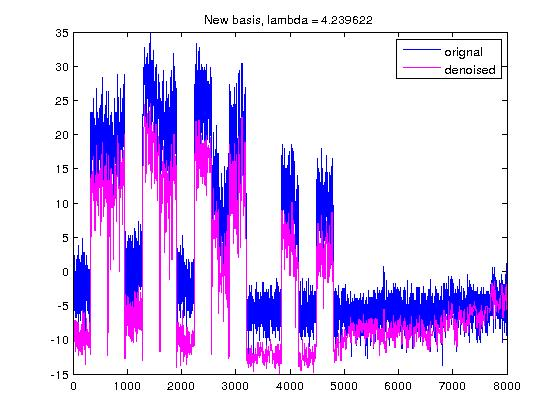
\includegraphics[height = 7.3 cm]{new_basis_ofcom_1.jpg}
\caption{}
\label{fig:hvb}
\end{figure}

\begin{figure}[h]
\centering
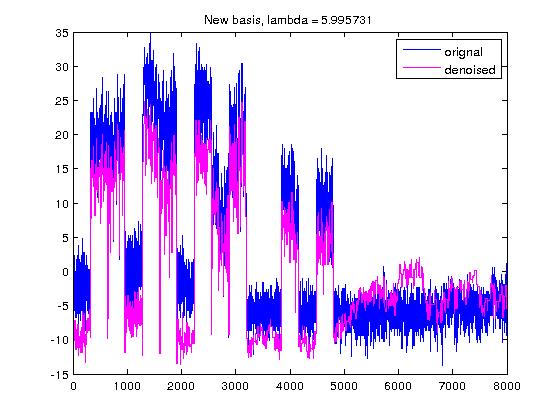
\includegraphics[height = 7.3 cm]{new_basis_ofcom_2.jpg}
\caption{}
\label{fig:hvb}
\end{figure}

\begin{figure}[h]
\centering
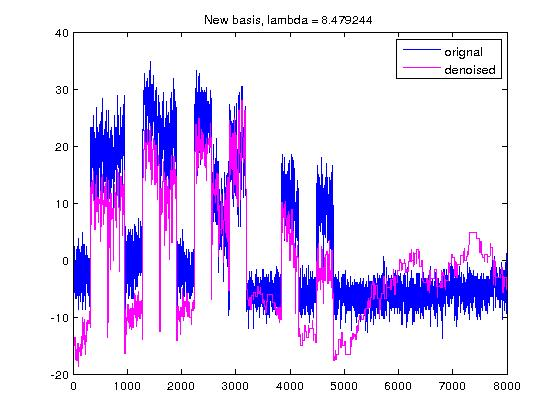
\includegraphics[height = 7.3 cm]{new_basis_ofcom_3.jpg}
\caption{}
\label{fig:hvb}
\end{figure}

\begin{figure}[h]
\centering
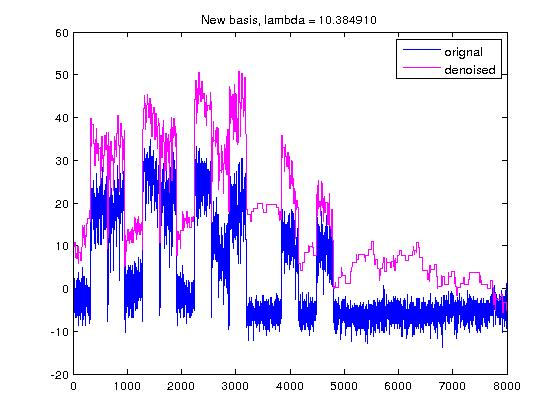
\includegraphics[height = 7.3 cm]{new_basis_ofcom_4.jpg}
\caption{}
\label{fig:hvb}
\end{figure}

These figures show that qualitatively, the distributed algorithm is capable of reconstructing the PSD in the TVWS band. These plots show that the trade off between reconstruction accuracy (in the mean square sense) and sparsity can be quite severe in this basis. We theorise that this is because of co-linearity between adjacent basis functions. This is a known feature of the lasso, and could possibly be alleviated by using a different reguluriser e.g. the OWL or OSCAR penalties. It is not clear that these penalties will be amenable to distributed implementation, however.

These plots show that a distributed network is in principle capable of performing large-scale reconstruction of PSD from compressive samples. In particular, no single node has access to the entire set of samples - so the compression rate per node could be quite severe. It should be noted that to our knowledge, this is the only study using data sets this size and with representative real-world data. 

\clearpage

\subsection{Compressive Estimation}

In this section, we apply display some examples of the output of procedure \ref{alg:single-shot}, as applied to the OFCOM data set. 

\begin{figure}[h]
\centering
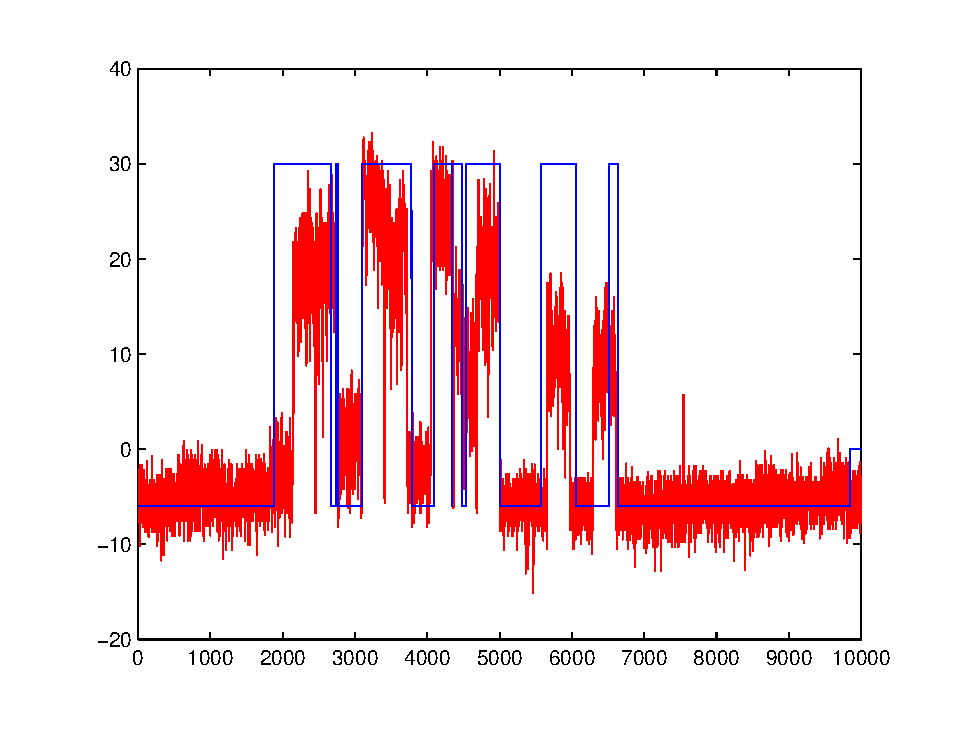
\includegraphics[height = 7.3 cm]{OFCOM5.eps}
\caption{Example of classification with OFCOM data, 35 changepoints}
\label{fig:hvb}
\end{figure}

\begin{figure}[h]
\centering
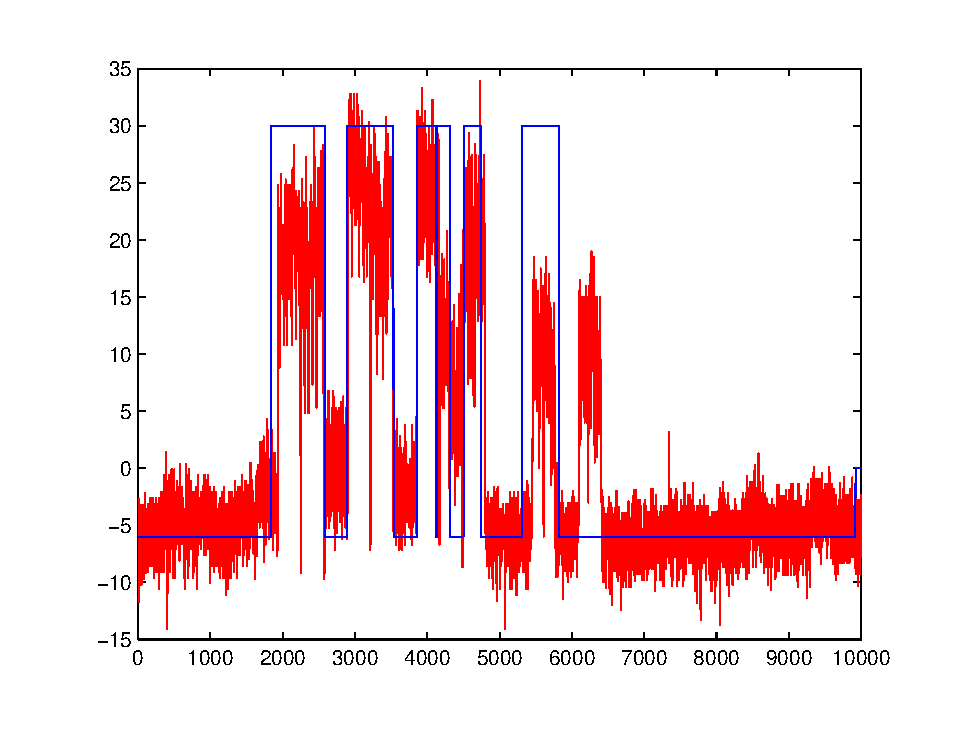
\includegraphics[height = 7.3 cm]{OFCOM6.eps}
\caption{Example of classification with OFCOM data, 85 changepoints}
\label{fig:hvb}
\end{figure}

\begin{figure}[h]
\centering
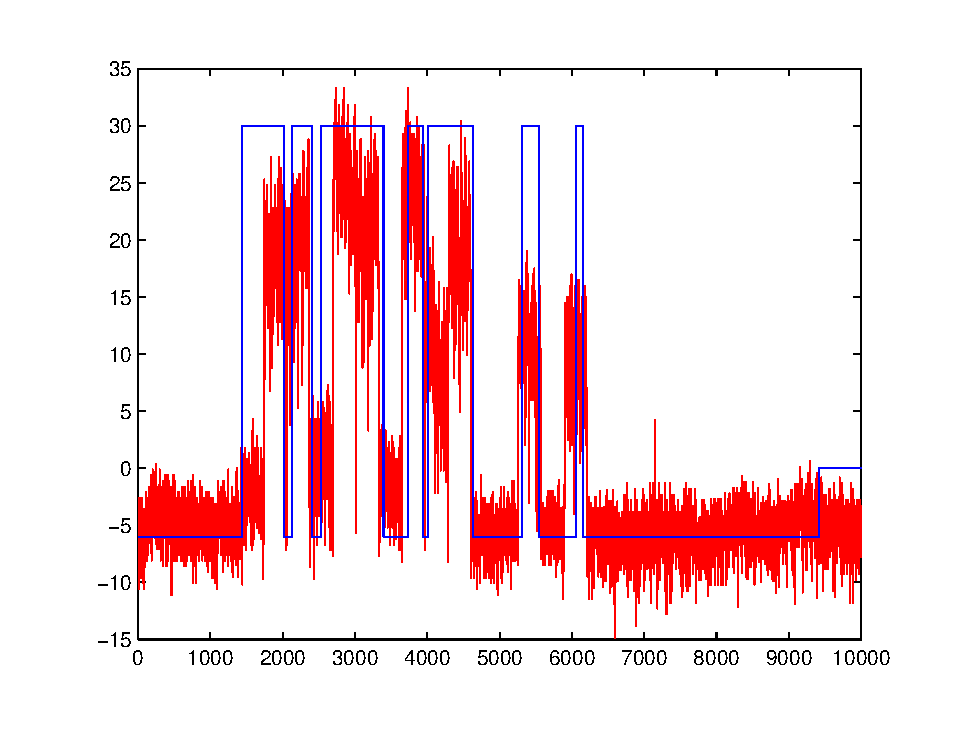
\includegraphics[height = 7.3 cm]{OFCOM7.eps}
\caption{Example of classification with OFCOM data, 55 changepoints}
\label{fig:hvb}
\end{figure}

\begin{figure}[h]
\centering
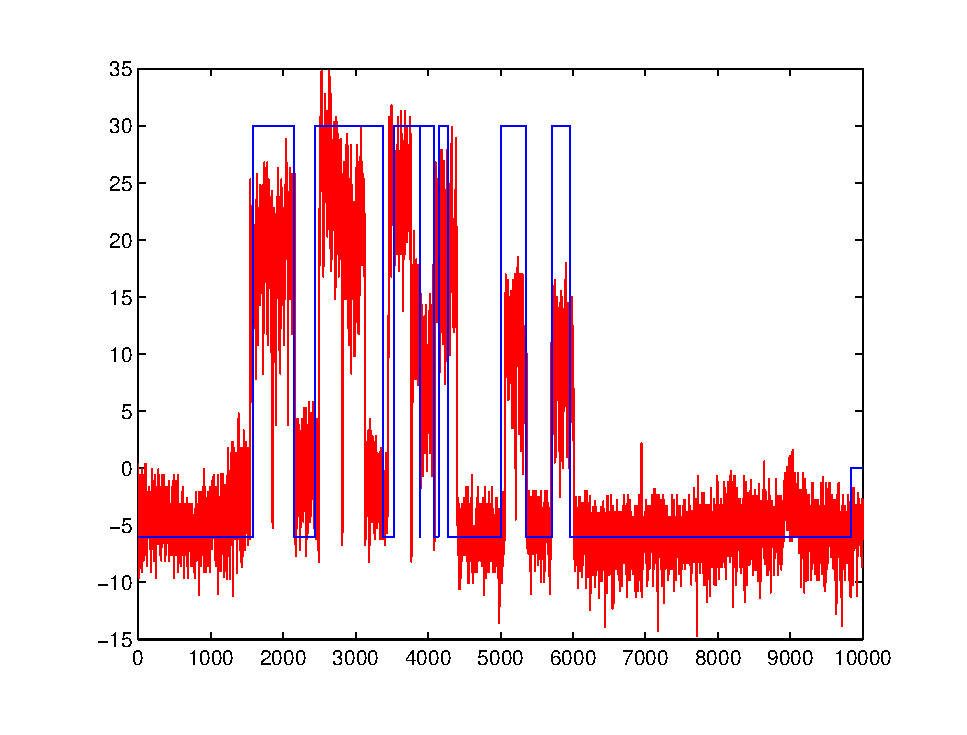
\includegraphics[height = 7.3 cm]{OFCOM8.eps}
\caption{Example of classification with OFCOM data, 55 changepoints}
\label{fig:hvb}
\end{figure}

These graphs show that the compressive estimation algorithm is capable of accurately classifying TVWS with datasets of this size. The accuracy of classification is highly dependent upon the number of changepoints used.
